\documentclass{book}

\usepackage{amsmath}
\usepackage{amssymb}
\usepackage{chemfig}
\usepackage{mathtools}
\usepackage{listings}
\usepackage{color}
\usepackage{wrapfig}
\usepackage{float}
\usepackage{caption}
\usepackage{fourier}
\usepackage{subcaption}
\usepackage{multicol}
\usepackage{paralist}
\usepackage{parskip}
\usepackage{tcolorbox}
\usepackage{tikz}
\usepackage{braket}
\usepackage[framemethod=TikZ]{mdframed}
\usepackage[english]{babel}
\usepackage[utf8x]{inputenc}
\usepackage[colorinlistoftodos]{todonotes}
\usepackage{esint}

\title{Research Notes}
\date{\today}
\author{Animesh Sinha}

\lstdefinestyle{shared}{
    belowcaptionskip=1\baselineskip,
    breaklines=true,
    xleftmargin=\parindent,
    showstringspaces=false,
    basicstyle=\fontsize{10}{6}\ttfamily,
}
\lstdefinestyle{cpp}{
	style=shared,
    language=C++,
    keywordstyle=\bfseries\color{green!40!black},
    commentstyle=\itshape\color{red!80!black},
    identifierstyle=\color{blue},
    stringstyle=\color{purple!40!black},
}
\lstdefinestyle{java}{
    style=shared,
    language=Java,
    keywordstyle=\bfseries\color{green!40!black},
    commentstyle=\itshape\color{purple!40!black},
    identifierstyle=\color{blue},
    stringstyle=\color{orange},
}
\lstdefinestyle{py}{
    style=shared,
    language=Python,
    keywordstyle=\bfseries\color{green!40!black},
    commentstyle=\itshape\color{purple!40!black},
    identifierstyle=\color{blue},
    stringstyle=\color{orange},
}
\lstdefinestyle{txt}{
    style=shared,
}
\lstset{escapechar=@}

\newcounter{theo}[section]\setcounter{theo}{0}
\renewcommand{\thetheo}{\arabic{section}.\arabic{theo}}
\newenvironment{theorem}[2][]{%
\refstepcounter{theo}%
\ifstrempty{#1}%
{\mdfsetup{%
frametitle={%
\tikz[baseline=(current bounding box.east),outer sep=0pt]
\node[anchor=east,rectangle,fill=blue!20]
{\strut Theorem~\thetheo};}}
}%
{\mdfsetup{%
frametitle={%
\tikz[baseline=(current bounding box.east),outer sep=0pt]
\node[anchor=east,rectangle,fill=blue!20]
{\strut Theorem~\thetheo:~#1};}}%
}%
\mdfsetup{innertopmargin=10pt,linecolor=blue!20,%
linewidth=2pt,topline=true,%
frametitleaboveskip=\dimexpr-\ht\strutbox\relax
}
\begin{mdframed}[]\relax%
\label{#2}}{\end{mdframed}}


\newcounter{trk}[section]\setcounter{trk}{0}
\renewcommand{\thetrk}{\arabic{section}.\arabic{trk}}
\newenvironment{trick}[2][]{%
\refstepcounter{trk}%
\ifstrempty{#1}%
{\mdfsetup{%
frametitle={%
\tikz[baseline=(current bounding box.east),outer sep=0pt]
\node[anchor=east,rectangle,fill=blue!20]
{\strut Trick~\thetrk};}}
}%
{\mdfsetup{%
frametitle={%
\tikz[baseline=(current bounding box.east),outer sep=0pt]
\node[anchor=east,rectangle,fill=blue!20]
{\strut Trick~\thetrk:~#1};}}%
}%
\mdfsetup{innertopmargin=10pt,linecolor=blue!20,%
linewidth=2pt,topline=true,%
frametitleaboveskip=\dimexpr-\ht\strutbox\relax
}
\begin{mdframed}[]\relax%
\label{#2}}{\end{mdframed}}


\newcounter{prf}[section]\setcounter{prf}{0}
\renewcommand{\theprf}{\arabic{section}.\arabic{prf}}
\newenvironment{proof}[2][]{%
\refstepcounter{prf}%
\ifstrempty{#1}%
{\mdfsetup{%
frametitle={%
\tikz[baseline=(current bounding box.east),outer sep=0pt]
\node[anchor=east,rectangle,fill=red!20]
{\strut Proof~\theprf};}}
}%
{\mdfsetup{%
frametitle={%
\tikz[baseline=(current bounding box.east),outer sep=0pt]
\node[anchor=east,rectangle,fill=red!20]
{\strut Proof~\theprf:~#1};}}%
}%
\mdfsetup{innertopmargin=10pt,linecolor=red!20,%
linewidth=2pt,topline=true,%
frametitleaboveskip=\dimexpr-\ht\strutbox\relax
}
\begin{mdframed}[]\relax%
\label{#2}}{\end{mdframed}}


\newcounter{exm}[section]\setcounter{exm}{0}
\renewcommand{\theexm}{\arabic{section}.\arabic{exm}}
\newenvironment{example}[2][]{%
\refstepcounter{exm}%
\ifstrempty{#1}%
{\mdfsetup{%
frametitle={%
\tikz[baseline=(current bounding box.east),outer sep=0pt]
\node[anchor=east,rectangle,fill=green!20]
{\strut Example~\theexm};}}
}%
{\mdfsetup{%
frametitle={%
\tikz[baseline=(current bounding box.east),outer sep=0pt]
\node[anchor=east,rectangle,fill=green!20]
{\strut Example~\theexm:~#1};}}%
}%
\mdfsetup{innertopmargin=10pt,linecolor=green!20,%
linewidth=2pt,topline=true,%
frametitleaboveskip=\dimexpr-\ht\strutbox\relax
}
\begin{mdframed}[]\relax%
\label{#2}}{\end{mdframed}}


\newcounter{def}[section]\setcounter{def}{0}
\renewcommand{\thedef}{\arabic{section}.\arabic{def}}
\newenvironment{definition}[2][]{%
\refstepcounter{def}%
\ifstrempty{#1}%
{\mdfsetup{%
frametitle={%
\tikz[baseline=(current bounding box.east),outer sep=0pt]
\node[anchor=east,rectangle,fill=yellow!20]
{\strut Definition~\thedef};}}
}%
{\mdfsetup{%
frametitle={%
\tikz[baseline=(current bounding box.east),outer sep=0pt]
\node[anchor=east,rectangle,fill=yellow!20]
{\strut Definition~\thedef:~#1};}}%
}%
\mdfsetup{innertopmargin=10pt,linecolor=yellow!20,%
linewidth=2pt,topline=true,%
frametitleaboveskip=\dimexpr-\ht\strutbox\relax
}
\begin{mdframed}[]\relax%
\label{#2}}{\end{mdframed}}


\newcounter{note}[section]\setcounter{note}{0}
\renewcommand{\thenote}{\arabic{section}.\arabic{note}}
\newenvironment{note}[2][]{%
\refstepcounter{note}%
\ifstrempty{#1}%
{\mdfsetup{%
frametitle={%
\tikz[baseline=(current bounding box.east),outer sep=0pt]
\node[anchor=east,rectangle,fill=pink!20]
{\strut Note~\thenote};}}
}%
{\mdfsetup{%
frametitle={%
\tikz[baseline=(current bounding box.east),outer sep=0pt]
\node[anchor=east,rectangle,fill=pink!20]
{\strut Note~\thenote:~#1};}}%
}%
\mdfsetup{innertopmargin=10pt,linecolor=pink!20,%
linewidth=2pt,topline=true,%
frametitleaboveskip=\dimexpr-\ht\strutbox\relax
}
\begin{mdframed}[]\relax%
\label{#2}}{\end{mdframed}}


\newcounter{algo}[section]\setcounter{algo}{0}
\renewcommand{\thealgo}{\arabic{section}.\arabic{algo}}
\newenvironment{algo}[2][]{%
\refstepcounter{algo}%
\ifstrempty{#1}%
{\mdfsetup{%
frametitle={%
\tikz[baseline=(current bounding box.east),outer sep=0pt]
\node[anchor=east,rectangle,fill=pink!20]
{\strut Algorithm~\thealgo};}}
}%
{\mdfsetup{%
frametitle={%
\tikz[baseline=(current bounding box.east),outer sep=0pt]
\node[anchor=east,rectangle,fill=pink!20]
{\strut Algorithm~\thealgo:~#1};}}%
}%
\mdfsetup{innertopmargin=10pt,linecolor=black,%
linewidth=2pt,topline=true,%
frametitleaboveskip=\dimexpr-\ht\strutbox\relax
}
\begin{mdframed}[]\relax%
\label{#2}}{\end{mdframed}}



\let\cleardoublepage\clearpage


\begin{document}
\pagenumbering{arabic}


\begin{titlepage}
    \newcommand{\HRule}{\rule{\linewidth}{0.5mm}}
    \center
    \textsc{\LARGE International Institute of Information Technology, Hyderabad}\\[1.5cm]
    
\includegraphics[scale=1]{img/iiit-logo.jpeg}\\[0.5cm]
    \textsc{\Large Machine Learning, Quantum Computation}\\[0.5cm]
    \textsc{\large Machine Learning and Physics in the vein of our primary work}\\[0.5cm] % Minor heading such as course title
    \HRule \\[0.4cm]
    { \huge \bfseries Research Notes}\\[0.4cm]
    \HRule \\[1.5cm]
    \begin{minipage}{0.4\textwidth}
        \begin{flushleft} \large
            \emph{Author:} Animesh Sinha
        \end{flushleft}
    \end{minipage}\\[2cm]
    {\large \today}\\[2cm]
    \vfill
\end{titlepage}

\tableofcontents

\chapter{Bayesian Machine Learning}


\section{What is Bayesian}


\section{Bayesian Linear Regression}


\section{Latent Variable Models}

Latent variable is one that we cannot observe.
\chapter{Reinforcement Learning}



\section{What is Reinforcement Learning}


\subsection{Constituents of a RL System}

\begin{itemize}
    \item Environment:
          Has an internal state $\bar{S_t}$ (true state), Takes an action $A_t$ and returns Observation $O_t$.
    \item Reward Signal:
          Takes the Observation $O_t$ to returns a reward $R_t$ not mutable by the agent.
    \item Agent (Learning algorithm):
          Has a State $S_t$, Value Function, Policy, Model (optionally).
\end{itemize}

Return is the sum of rewards over all steps: $G_t = G_{t − 1} + R_t$.

The goal is to maximize the following:
\begin{equation}
    q(s, a) = E[G_t ∣ S_t = s, A_t = a] = E[R_{t_1} + R_{t_2} + \dots ∣ S_t = s, A_t = a]
\end{equation}


\subsection{Terms relation to the state}

\subsubsection{State of the Environment}

History is defined to be the set of all actions and observations with which we can recreate the current state: $ H_t = A_0 O_0 A_1 O_1 \dots A_n O_n $

Fully Observable State are defined to have: $S_t = O_t$, that is the current observation represents the entire state of the game.

For Partially observable environments, we can represent the state using a Recurrent Neural Network with Memory to store some features of the history.

The state may be Markovian only to the environment and not to the agent, if there are additional unknows for the agent.

\begin{definition}[Markov Decision Process]{def:mdp}
    A decision process is Markovian if: $p(r, s ∣ S_t, A_t) = p(r, s ∣ H_t, A_t)$, i.e. the future is independent of the part given the present ($H_t \rightarrow S_t \rightarrow H_t+1$).
\end{definition}

One of the reasons why an environment is not Markov is because it's non-stationary (and we don't want to or can't model how the environment evolved)

\subsubsection{State of the Agent}

\begin{theorem}[Bellman Equations]{thm:bellman-equations}
    \begin{eqnarray}
        v_\pi &=& E[E_t + 1 + \gamma G_t + 1 ∣ S_t = s, A_t \sim \pi(s)] \\
        &=& E[E_t + 1 + \gamma v_\pi(S_t+1) ∣ S_t=s, A_t \sim \pi(s)]
    \end{eqnarray}
\end{theorem}

The same holds true for the optimal value function (this equation is independent of the policy):
\begin{equation}
    v_∗ = max_a[E_t + 1 + \gamma v_∗ G_t + 1 | S_t = s, A_t = a]
\end{equation}
Agents often approximate the value function.

\subsubsection{Model of the Environment}

Transition probabilities:
\begin{equation}
    P(s, a, s^\prime) = P(S_t + 1 = s^\prime ∣ S_t = s, A_t = a)
\end{equation}

Immediate reward:
\begin{equation}
    R(s, a) = E[R_t + 1 ∣ S_t = s, A_t = a]
\end{equation}



\section{Exploration and Exploitation}

\emph{In this section we are taking the example of the Multi-Arm Bandit, the major assumption is that the length of the episode is 1, our actions do not affect our state.}

The true value of the action is: $q(a) = E[R_t | A_t = a]$.
\begin{note}[Q-Value Update]{note:q-value-update}
    We have an approximation on the value, we can update as follows:
    \begin{eqnarray}
        Q_t(a) &=& \frac{\sum_{n=1}^{t} R_n I(A_n = a)}{\sum_{n=1}^{t} I(A_n = a)} \\
        Q_t(A_t) &=& Q_{t-1}(A_t) + \alpha_f(R_f - Q_{t-1}(A_t))
    \end{eqnarray}
\end{note}


\subsection{Lower Bound on Regret}

Regret is the value by which we got the rewards wrong:
\begin{equation}
    G = \sum_t (v_* - q(A_t)) = \sum_a N(a) (v_* - q(a))
\end{equation}
We want to minimize the regret over the training-cum-test period (we can forever keep learning).

If we use methods like $\epsilon$-Greedy (explore some times and exploit other times), our regret growth is still linear in the length of time, which is only constant factor better from learning nothing.

We can prove the lower bound that Asymptotic total regret is at least Logrithmic in the number of steps. This is formally described by the gap $\Delta_a = (v_* - q(a))$.
\begin{equation}
    \lim_{t \rightarrow \infty} L_t \geq log(t) \sum_{a \vert \Delta_a > 0} \frac{\Delta_a}{KL(p(r \vert a) \Vert p(r \vert a_*))}
\end{equation}
The regret is still unbounded, but it's lower-bounded by logrithm in $t$.


\subsection{Upper Confidence Bound}

\textbf{Hoeffding's Inequality} is a concentration bound result. Given independent and identically distributed random variables $X_1, X_2, \dots X_n$, let $\bar{X} = \frac{1}{n} \sum_{i=1}^{n} X_i$ be the sample mean. Then:
\begin{equation}
    p((\mathbb{E}[X] - \bar{X}) < u) = e^{-2nu^2}
\end{equation}

If we assume that are rewards are in the range [0, 1), then we can derive the relation for the upper confidence bound for probability p (the maximum range we can be sure the rewards are in with probability atleast p):
\begin{eqnarray*}
    p(q(a) \geq Q_t(a) + U_t(a)) &\leq& e^{-2N_t(a)U_t(a)^2} \\
    \implies U_t(a) &=& \sqrt{\frac{-\log(p)}{2N_t(a)}}
\end{eqnarray*}
The root over the number of observations is due to the assumptions that the variables are IID, using central limit theorem our confidences are gaussians, the standard deviation for it is proportional to root of n.

We want to set p increasing proportionally to time. So we can replace p with n.

\begin{algo}[UCB algorithm]{algo:ucb-algo}
    \begin{equation}
        a_t = argmax_{a \in \mathcal{A}} Q_t(a) + c\sqrt{\frac{log t}{N_t(a)}}
    \end{equation}
    c is a hyperparameter which represent learning rate of some sort (usually 1 to 2).

    Setting $c = \sqrt{2}$, the Logrithmic lower bound (upto constant) is achieved. $L_t \leq 8 \sum_{a \vert \Delta_a > 0} \frac{log(t)}{\Delta_a} + O(\sum_a \Delta_a)$.
\end{algo}


\subsection{Model-Based Bayesian Bandits}

Bayesian Bandit models are parametrized distributions over rewards $P(R_t \vert \theta, a)$, for each action a given some parametrization of our model $\theta$ (like mean and variance of Gaussian, etc, based on belief state of model).
\begin{equation}
    p_t(\theta | a) \propto p(R_t | \theta, a) p_{t-1}(\theta | a)
\end{equation}
Parameters $\Theta$ are being used to learn the true value of the reward, and we can inject our prior knowledge into $p_{0}(\theta | a)$.

\begin{figure}[H]
    \centering
    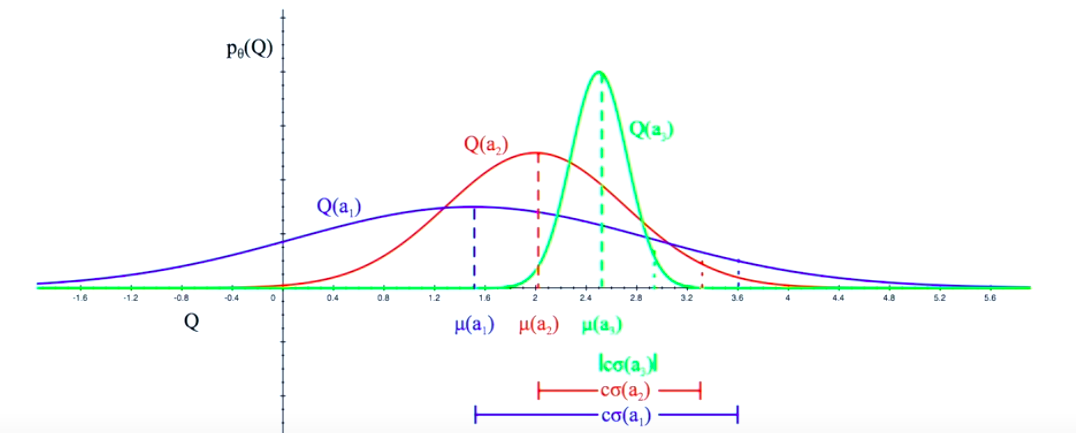
\includegraphics[width=\linewidth]{img/rl/ucb-bandits.png}
    \caption{Example of the Bayesian Beliefs over Reward}
    \label{fig:ucb-bayesian-bandits}
\end{figure}

If we have the case of Bernouli bandits, we can use the Beta distributions, which will be parametrized by the number of times we have gotten a zero and a one, i.e. $Q_t(a) = \beta(N_t(R = 0 | a), N_t(R = 1 | a))$.

Computing the posterior may be a lot harder for general examples. We have several ways to solve for the correct action given the posterior distributions.

\subsubsection{Upper Confidence Bound - Bayesian}

\begin{itemize}
    \item We compute the Posterior over the action values ($p(R_t | \theta, a)$)
    \item We pick an upper confidence bound, eg. standard deviation ($U_t(a) = \sigma$)
    \item We act in a way that maximizes $Q_t(a) + U_t(a)$
\end{itemize}

\subsubsection{Probability Matching}

We will select each action with the probability of it being optimal.
\begin{equation}
    \pi_t(a) = p(q(a) = max_{a^\prime} q(a^\prime) \vert H_{t-1})
\end{equation}
The probability may be difficult in general to get this probability analytically.

\subsubsection{Thomson Sampling}

We try to sample from the probability over the reward of each actions, and then select greedily.
\begin{equation}
    \pi_t(a) = \mathbb{E}[\mathcal{I}(Q_t(a) = max_{a^\prime} Q_t(a^\prime))] = p(q(a) = max_{a^\prime} q(a^\prime))
\end{equation}
This achives the Logrithmic lower bound of regret.

\subsubsection{Information State Space}

If we can quantify the value of information gained in terms of future rewards that we gain given the information. This is a Markov Decision Process over the internal observation states. (We will need to know $p(\tilde{s^\prime} \vert a, \tilde{s})$).
\begin{itemize}
    \item Solvable using Model Free Reinforcement Learning (Q-Learning)
    \item Solvable using Model Based Bayesian Reinforcement Learning (Gittens Indices)
\end{itemize}
This can be unwieldy and not scalable.


\subsection{Policy Based Methods}

Below is the definition of the policy, soft-max over action values, where the values H are just preferences and do not bear a direct correspondance to the action/state values.
\begin{equation}
    \pi(a) = \frac{e^{H_t(a)}}{\sum_b e^{H_t(b)}}
\end{equation}
Now we want to do gradient ascent over the value of the rewards, updating our preferences.
\begin{equation}
    \theta = \theta + \alpha \nabla_\theta \mathbb{E}[R_t | \theta]
\end{equation}


\begin{theorem}[Log Likelihood trick]{thm:log-likelihood-trick}
    We are computing the gradient for the Bandits, this is also known as the Reinforce trick (Williams, 1992).
    \begin{eqnarray}
        \nabla_\theta \mathbb{E}[R_t \vert \theta]
        &=& \nabla_\theta \sum_a \pi_\theta(a) \mathbb{E}[R_t \vert A_t = a] \\
        &=& \sum_a q(a) \nabla_\theta \pi_\theta(a) \\
        &=& \sum_a q(a) \frac{\pi_\theta(a)}{\pi_\theta(a)} \nabla_\theta \pi_\theta(a) \\
        &=& \sum_a \pi_\theta(a) q(a) \frac{\nabla_\theta \pi_\theta(a)}{\pi_\theta(a)} \\
        &=& \mathbb{E}[R_t \frac{\nabla_\theta \pi_\theta(A_t)}{\pi_\theta(A_t)}] \\
        &=& \mathbb{E}[R_t \nabla_\theta log \pi_\theta(A_t)] \\
    \end{eqnarray}
    We have converted a gradient over expectation into an expectation over a gradient, so now we can sample from the gradient of the distribution to be able to perform stochastic gradient descent.
\end{theorem}

Stochastic Gradient Ascent is now $\mathbf{\theta = \theta + \alpha R_t \nabla_0 log(\pi_0(A_t))}$

In the case of SoftMax over action preferences, we have:
\begin{eqnarray}
    H_{t+1}(a) &=& H_t(a) + \alpha R_t \frac{\partial log \pi_t(A_t)}{\partial H_t(a)} \\
    &=& H_t(a) + \alpha R_t (\mathcal{I}(a = A_t) - \pi_t(a)) \\
    \implies H_{t+1}(a) &=& H_t(a) + \alpha R_t \times \begin{cases}
        (1 - \pi_t(a)) \; \text{if}\; a = A_t \\
        (-\pi_t(a)) \; \text{if}\; a \neq A_t
    \end{cases}
\end{eqnarray}
So we are increasing the preferences of actions with higher rewards and pushing down the preferences of the actions even without taking them, therefore it's not the same as value.

We also note that the sum of probabilities over all actions is always 1, so we can add a baseline (constant independent of $\theta$ and $a$) to the reward without changing the preferences. But it does change the variance of the update. So
\textbf{performance can improve by adding a baseline like negative of the mean till now}.

\section{Dynamic Programming to solve MDPs}

The discount factor affects the goal we are going after.

\chapter{Basic Neural Network Architectures in Keras}

\section{Common Code for Neural Nets}


\subsection{Train models with Saved intermediates}


Following is the basic code to run when training the neural Network.

\begin{lstlisting}[style=py]
model.fit(x=X_train, y=X_train, epochs=25,
validation_data=[X_validation, Y_validation],
callbacks=[keras_utils.ModelSaveCallback(model_filename),
        keras_utils.TqdmProgressCallback()],
verbose=0,
initial_epoch=last_finished_epoch or 0)
\end{lstlisting}

And this is the code to load a presaved checkpoint of the model and start traininf from the last completed epoch. The keras\_utils file is available in the snippets, and makes these callbacks available.

\begin{lstlisting}[style=py]
def load_checkpoint(last_epoch)
    model_filename = 'model.{0:03d}.hdf5'
    last_finished_epoch = None
    if last_epoch is not None:
        s = keras_utils.reset_tf_session()
        last_finished_epoch = 4
        model = keras.models.load_model(model_filename.format(last_finished_epoch))
\end{lstlisting}

Following this, we always save our weights in a file, and then load from it, as follows:
\begin{lstlisting}[style=py]
encoder.save_weights("encoder.h5")
decoder.save_weights("decoder.h5")
\end{lstlisting}



\section{AutoEncoders}

\subsection{Convolutional Autoencoders}

Here is the code for the setting up a Convolutional AutoEncoders. Follows a 4 layer Conv-Pool and then 1 Dense layer architecture to encode, then a dense layer followed by Transpose Convolutional layers to decode.

\lstinputlisting[style=py]{snippets/ml_architectures/convolutional_autoencoder.py}



\section{Recurrent Units}


\subsection{Long Short Term Memory (LSTM)}

\subsubsection{Schematic Sketch}

\begin{figure}[H]
	\centering
	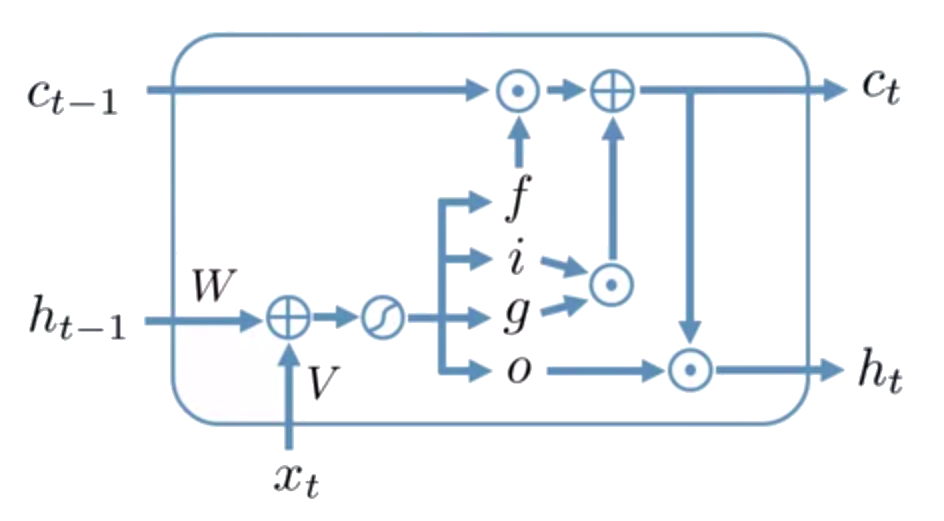
\includegraphics[width=0.9\linewidth]{img/aml/lstm-schematic.png}
	\caption{Schematic Diagram of LSTM}
	\label{fig:lstm-schmatic}
\end{figure}

\subsubsection{Update Equations}

Following are the update equations for an LSTM. There are 3 gates, the Input Gate (which saves to cell memory), and Output Gate (which loads from cell memory) and a Forget Gate (which clears up cell memory). In addition a Gate Value is generated, which is what gets stored in the memory during input. All these get computed from the catenation of the previous hidden state and the current input.

\begin{eqnarray}
	g_t &=& \tilde{f}(W_g \cdot \text{Concat}[x_t, h_{t - 1}] + b_g) \\
	f_t &=& \sigma(W_f \cdot \text{Concat}[x_t, h_{t - 1}] + b_f) \\
	i_t &=& \sigma(W_i \cdot \text{Concat}[x_t, h_{t - 1}] + b_i) \\
	o_t &=& \sigma(W_o \cdot \text{Concat}[x_t, h_{t - 1}] + b_o) \\
	c_t &=& f_t \cdot c_{t - 1} + i_t \cdot g_t \\
\end{eqnarray}

The hidden state is the output, which can be available as the entire sequence or only at the end. A dense layer or any other can be used on top of it to compute some other output $y_t$.

\subsubsection{Management of Gradients}

Since the memory cell connections are like a skip connection if there is no update/forget operation, the gradients do not vanish as easily.


\subsection{Gated Recurrence Unit (GRU)}

\subsubsection{Schematic Sketch}

\begin{figure}[H]
	\centering
	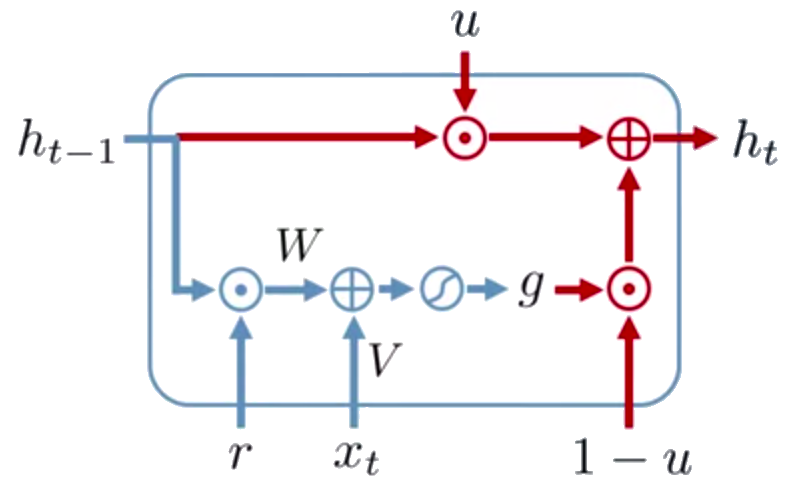
\includegraphics[width=0.9\linewidth]{img/aml/gru-schematic.png}
	\caption{Schematic Diagram of GRU}
	\label{fig:gru-schmatic}
\end{figure}

\subsubsection{Update Equations}


\chapter{Particle Physics for Data Scientists}



\section{The Preliminaries}


\subsection{Problems with the standard model}

What makes us unhappy?
\begin{itemize}
  \item Matter and Antimatter inequivalence.
  \item 19 Arbitrary constants.
  \item Why is Gravity so weak.
\end{itemize}


\subsection{The Particles we want to detect}

\begin{figure}[H]
  \centering
  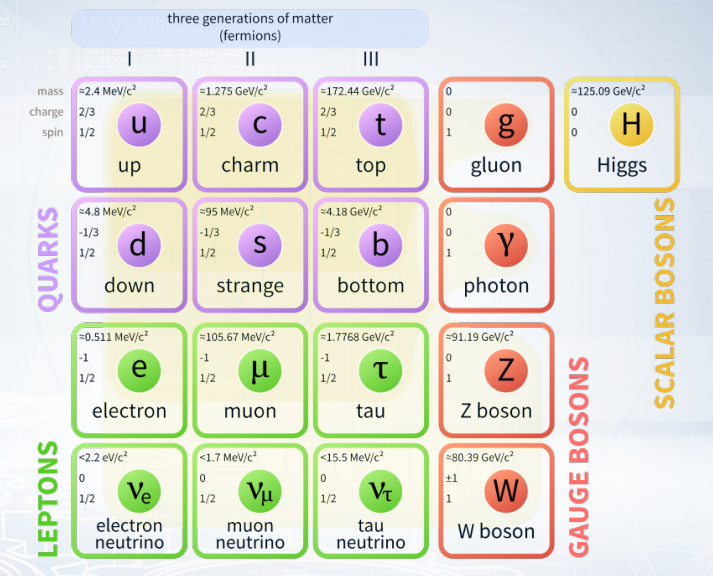
\includegraphics[width=0.4\linewidth]{img/hadron/particleid-list.png}
  \caption{List of Particles of different types}
  \label{fig:particleid-list}
\end{figure}

The following are types of particles we want to defect.
\begin{multicols}{3}
  \begin{itemize}
    \item muon
    \item kon
    \item pion
    \item proton
    \item electron
  \end{itemize}
\end{multicols}



\subsection{The Experiments in LHC}

There are 4 major detectors
\begin{itemize}
  \item ALICE (A Large Ion Collider Experiment) is a heavy-ion detector on the Large Hadron Collider (LHC) ring. It is designed to study the physics of strongly interacting matter at extreme energy densities, where a phase of matter called quark-gluon plasma forms.
  \item ATLAS (A Toroidal LHC ApparatuS) is one of two general-purpose detectors at the Large Hadron Collider (LHC). It investigates a wide range of physics, from the search for the Higgs boson to extra dimensions and particles that could make up dark matter. Although it has the same scientific goals as the CMS experiment, it uses different technical solutions and a different magnet-system design. It has a cylindrical structure and measures particles in all directions.
  \item CMS (Compact Muon Solenoid) is a general-purpose detector at the Large Hadron Collider (LHC). It has a broad physics programme ranging from studying the Standard Model (including the Higgs boson) to searching for extra dimensions and particles that could make up dark matter. Although it has the same scientific goals as the ATLAS experiment, it uses different technical solutions and a different magnet-system design.
  \item LHCb (Large Hadron Collider Beauty) experiment specializes in investigating the slight differences between matter and antimatter by studying a type of particle called the "beauty quark", or "b quark". It is a single arm forward spectrometer.
\end{itemize}

We smash bunches of protons ('events'), record the pixels ('hits'), reconstruct trajectories ('jets', 'showers', 'tracks'), and we perform Statistical analysis on them.

A Trigger System is a system that uses criteria to rapidly decide which events in a particle detector to keep when only a small fraction of the total can be recorded.


\subsection{Simulation Package}

\begin{itemize}
  \item http://www.genie-mc.org/
  \item http://home.thep.lu.se/Pythia/: Nutrino Simulations
  \item GEANT4: http://geant4.web.cern.ch/: Particles interacting with matter.
  \item FLUKA: http://www.fluka.org/fluka.php
\end{itemize}


\subsection{Feynman Diagrams}

\begin{figure}[H]
  \centering
  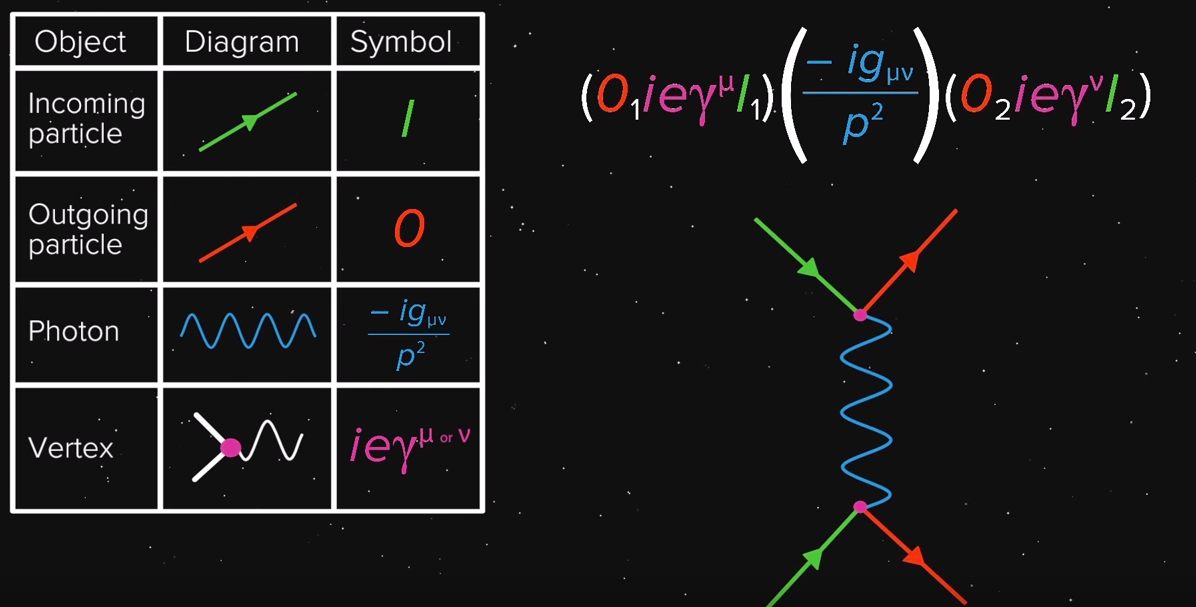
\includegraphics[width=0.8\linewidth]{img/hadron/preliminary-feynman-diagram.png}
  \caption{A Sample Feynman Diagram for scattering of Two electron by the transfer of one Photon}
  \label{fig:preliminary-feynman-diagram}
\end{figure}



\section{The Large Hadron Collider Setup}

\begin{figure}[H]
  \centering
  \begin{subfigure}[b]{0.5\textwidth}
    \centering
    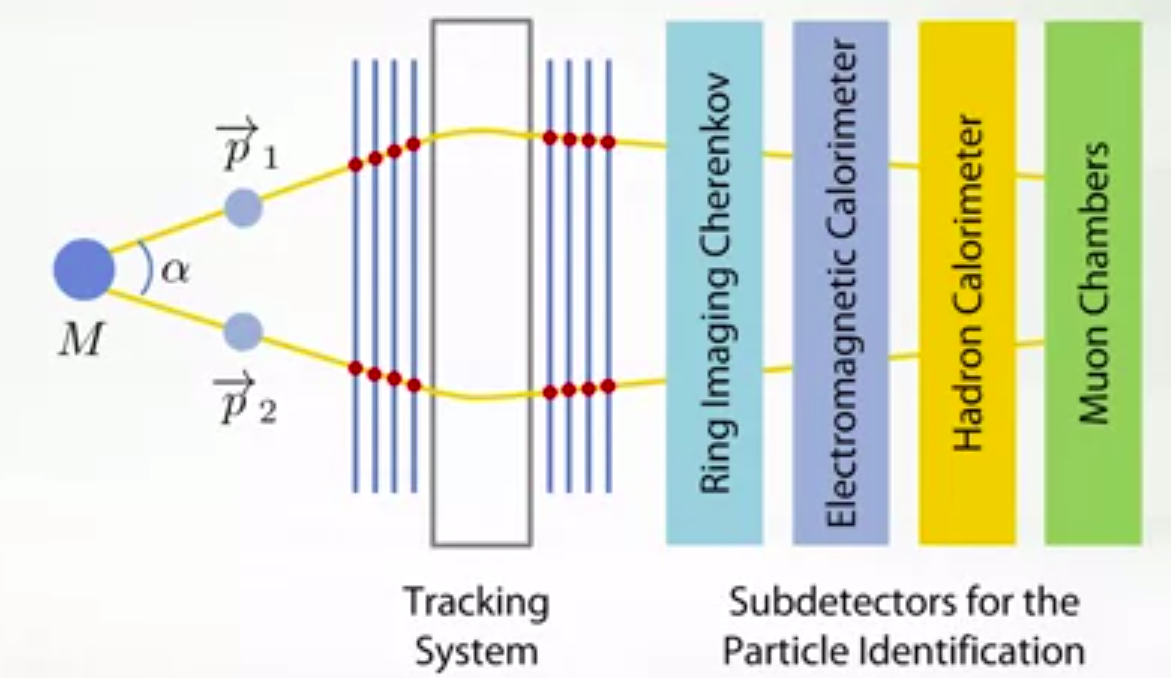
\includegraphics[width=\linewidth]{img/hadron/particleid-detector-setup.png}
    \caption{Detector Setup of the LHC}
    \label{fig:particleid-detector-setup}
  \end{subfigure}
  \begin{subfigure}[b]{0.4\textwidth}
    \centering
    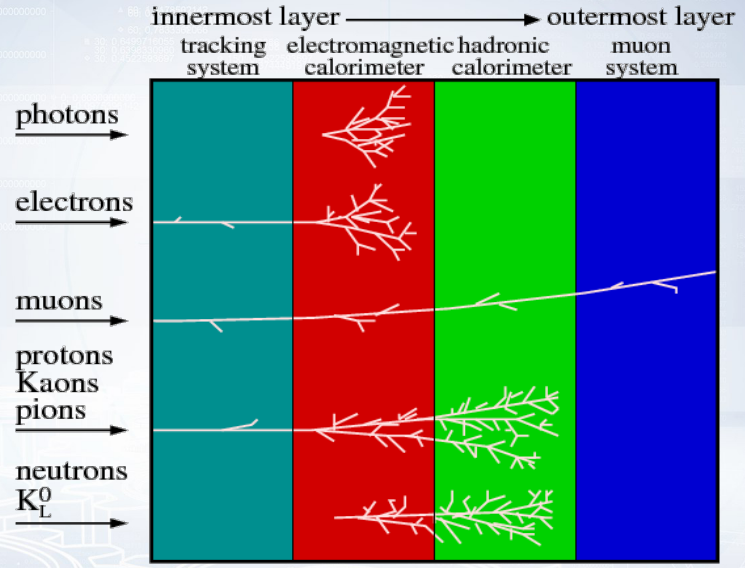
\includegraphics[width=\linewidth]{img/hadron/particleid-tracking.png}
    \caption{The tracks made in the Chambers}
    \label{fig:particleid-tracking}
  \end{subfigure}
\end{figure}


\subsection{Tracking System}

The first system of detectors, stands before particle collision area. Important for parameter estimation. 

There are several layers of sensors that measure hits, and allow us to recognise particle trajectories.
There is also a Magnetic Field that allows us to measure momentum (using radius of curvature in the field).

We have the following conservation equationsm wgeb a particle $D^0$ with mass $m$ breaks into a $K^-$ with mass $m_1$ and a $\pi^+$ with mass $m_2$, and they go away from each other at angle $\alpha$:
\begin{eqnarray}
  E_m &=& E_1 + E_2 \\
  \hat{p_m} &=& \hat{p_1} + \hat{p_2} \\
  E^2 &=& p^2 c^2 + m^2 c^4 \\
  M^2 &=& m_1^2 + m_2^2 + \frac{2}{c^4} (E_1 E_2 - p_1 p_2 c^2 cos\alpha)
\end{eqnarray}

\subsubsection{Problem: Track Pattern Recognition} Recognizing hits that belong to the same track. Currently we have the following methods.
\begin{itemize}
  \item Half Transform and Kalman Filtering. (Statistical, computationally cheaper.)
  \item Hopfield Neural Netorks. (Denby Peterson and Cellular Automaton.)
  \item Convolutional Nerual Networks (classify result as correct or wrong). Recurrent Neural Netorks (predict the next hit location).
\end{itemize}
We can then combine these particle tracks into decays.

\subsection{Ring Imaging Chernekov Detector (RICH)}

This is the first detector because it does not affect the flight of the particle.

\begin{figure}[H]
  \centering
  \begin{subfigure}[b]{0.45\textwidth}
      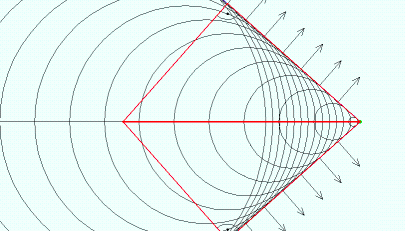
\includegraphics[width=\linewidth]{img/hadron/particleid-chernekov-wavefronts.png}
      \caption{Chernekov Simulation}
  \end{subfigure}
  \begin{subfigure}[b]{0.30\textwidth}
      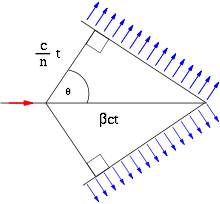
\includegraphics[width=\linewidth]{img/hadron/particleid-cherenkov-angles.png}
      \caption{Chernekov Angles}
  \end{subfigure}
  \begin{subfigure}[b]{0.45\textwidth}
    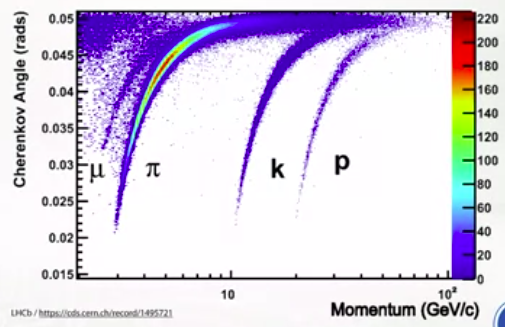
\includegraphics[width=\linewidth]{img/hadron/particleid-chernekov-graph.png}
    \caption{Chernekov Radiation Graphs}
  \end{subfigure}
  \label{fig:particleid-chernekov-wavefronts}
  \caption{Registers in Processor Design}
\end{figure}

Here is the angle of the Chernokov radiation, derivable using simple geometric means and some special relativity in terms of the momentum.
\begin{equation}
  p = \frac{mc\beta}{\sqrt{1 - v^2/c^2}}
\end{equation}
\begin{equation}
  cos \theta = \frac{1}{n\beta} = \frac{\sqrt{p^2 + m^2c^2}}{np}
\end{equation}
From the figure above, and the equation for it's analytical feel, that we can figure out the mass of the particle and thereby which particle it is.

% ISSUE: 5:40 Kaon and Pion rings.

\subsection{Calorimeter - Electromagnetic and Hadronic}

Electromagnetic stops all but than muons and quarks. Hadron calorimeter stops the quarks.

\begin{equation}
  E_C = E_0 e^{\frac{x}{X_0}}
\end{equation}
\begin{equation}
  X_{max} = X_0 ln(\frac{E_0}{E_c})
\end{equation}
\begin{equation}
  N = E_0 / E_c
\end{equation}

After this we have crystals and scintillation counters, that measure the count and energy of particles, The electrons and photons, and since we measure energy, we already have momenta from the tracking system., this gives us the Mass, so we can identify them.

\subsection{Muon Chambers}

Muons do not interact well with matter. So we have multiple layers of metal to slow down the muons, they activate the chambers, we will extrapolate the data to get which particles in the tracking system were muons. We can also get the energy from how far they go in the muon chambers.


\subsection{How to make a classifier uniform}

\subsubsection{The problem}
\begin{eqnarray}
1 - false\;positive\;rate &=& background\;rejection \\
true\;positive\;rate &=& signal\;efficiency
\end{eqnarray}
We want to have no dependence of the ROC AUC on all the momenta.

\begin{eqnarray}
  L_{ada} &=& \Sigma e^{-\gamma_i S_i} \\
  L_{flat} &=& \Sigma_b w_b \int |F_b(s) - F(s)|^2 ds \\
  L_{adaflat} &=& L_{ada} + \alpha L_{flat}
\end{eqnarray}
This is imposing an additional loss over the ADA boost function to make it less dependent on the momentum, alpha is a parameter we can tune to weight flatness over fit quality.

\subsection{Adversarial Neural Networks}

Minimizing dependencies on Mass, Momentum, etc. can also be done using adversarial neural networks. One network performs classification, and feeds it's output to the other which tries to guess the momentum/mass from the output, if it can do this well, the model is bad, i.e. not flat. So, our new loss is $Loss_{classification} + f(Loss_{adversarial})$.


\section {Discovering New Physics}

% TODO: Learn about different classes of Particles in Standard model, SUSY Particles
% Particle-Data-Group has breaking of all particles

\subsection{NoEther's theorem}

NoEther's theorem claims that the conservation laws we have are based on certain symetries.
Here is a list of some of them.
\begin{itemize}
  \item Time Inversion: Energy
  \item Space Translation: Linear momentum
  \item Space Rotation: Angular momentum
  \item Charge Conjugation and Parity: Time Isotropy
  \item Charge, Lepton Number: Gauge Symetries 
\end{itemize}

\subsection{}

CvM test 
\begin{equation}
  CvM = \Sigma_{region} \int |F_{region}(s) - F_{global}(s)|^2 dF_{global}(S)
\end{equation}

% UBoost BDT

\subsection{Doping}


\chapter{Group Theory and Graphs}



\section{Groups and Subgroups}

\subsection{What is a Group?}
A group is defined over a Set A and an arbitrary operation $\times$, denoted as: $\braket{A|\times}$.
\begin{itemize}
    \item \textbf{Closure:} If a and b are elements in A, then $a \times b$ is also in A.
    \item \textbf{Identity:} There exists e such that $a \times e = a$.
    \item \textbf{Invertability:} There exists $a^{-1}$ such that $a \times a^{-1} = e$.
    \item \textbf{Associativity:} $(a \times b) \times c = a \times (b \times c)$
\end{itemize}

A Subgroup is a subset of the original group that is itself a group.
\paragraph{One Step Subgroup Test} states that if $ab^{-1}$ is in the group H, then H is a subgroup of G.
\paragraph{Two Step Subgroup Test} states that if $a^{-1}$ is in H whenever a is in H and $ab$ is in H for all a, b in H, then H is a subgroup of G.
\paragraph{Finite Subgroup Test} If H is a non-empty finite subset of a group G, and H is closed under the operation G, then H is a subgroup of G.

\paragraph{Operations that Hold} in groups are:
\begin{itemize}
    \item Uniqueness of Identity (If $ x \cdot a = x $ and $ x \cdot b = x $, $(\forall x)$, then $a = b = e$)
    \item Uniqueness of Inverse (If $ x \cdot a = e $ and $ x \cdot b = e $, $(\exists x)$, then $a = b = x^{-1}$)
    \item Left and Right Cancellation (If $ab = ac$ then $b = c $. If $ba = ca$ then $b = c$.)
    \item Socks-Shoes Property ($(ab)^{-1} = b^{-1} a^{-1}$)
\end{itemize}


\subsection{Cayley's Table}

\paragraph{Cayley's Table} is a 2-D matrix of all members of the group $a$ and $b$ on both axis and $a \cdot b$

\subsection{Subgroups and GCD}

\begin{theorem}[Equivalent Cyclic Subpgroups]{thm:groups-cyclic-gcd}
    Let a be an element of order n in a group and let k be a positive integer. Then
    \colorbox{yellow}{$ \braket{a^k} = \braket{a^{gcd(n,k)}}\;and\;|a^k| = n/gcd(n, k). $}
\end{theorem}

\begin{proof}[Equivalent Cyclic Subpgroups]{prf:groups-cyclic-gcd}
    $(a^{gcd(n,k)})^{\alpha} = a^k$, Since gcd(n,k) divides k. Thereby $ \braket{a^{k}} \subseteq \braket{a^{gcd(n,k)}}$.
    Also, $gcd(n,k) = \alpha n + \beta k$, so $a^{gcd(n,k)} = a^{\alpha n + \beta k} = a^{\alpha n} a^{\beta k} = e \cdot a^{\beta k}$, therefore we can state that, $\braket{a^{gcd{n,k}}} \subseteq \braket{a^k}$. So we proved that $\braket{a^k} = \braket{a^{gcd(n,k)}}$.
    \vspace{10pt} \\ Next, using the proof in the first part, since the groups are equal their orders are the same, so
    $|a^{k}| = |a^{gcd(n,k)}| = \frac{n}{gcd(n,k)}$, since the gcd divides n, it is the least solution to $(a^{gcd(n,k)})^x = a^n$
\end{proof}

This has the following crucial corollaries.
\begin{itemize}
    \item In a finite cyclic group, the order of an element divides the orderof the group.
    \item Let $|a| = n$. Then $\braket{a^i} = \braket{a^j}$ if and only if $gcd(n, i) = gcd(n, j)$, and $|a^i| = |a^j|$ if and only if $gcd(n, i) = gcd(n, j)$.
    \item Let $|a| = n$. Then \colorbox{yellow}{$\braket{a} = \braket{a^j}$ if and only if $gcd(n, j) = 1$}, and $|a| = |\braket{a^j}|$ if and only if $gcd(n, j) = 1$.
    \item An integer k in $Z_n$ is a generator of $Z_n$ if and only if $gcd(n, k) = 1$.
\end{itemize}
These facts help us count the number of subgroups in a given set.


\subsection{Cyclic Groups}

\begin{theorem}[Fundamental Theorem of Cyclic Groups]{thm:groups-FundamentalTheoremCyclicGroups}
    Every subgroup of a cyclic group is cyclic.
    Moreover, if $|\braket{a}|$ = n, then the order of any subgroup of $\braket{a}$ is a divisor of n; and, for each positive divisor k of n, the group $\braket{a}$ has exactly one subgroup of order k, namely, $\braket{a^{n/k}}$.
\end{theorem}

\begin{theorem}[Number of Elements of Order D]{thm:groups-OrderD}
    Let $G_n$ be a finite Cyclic Group of order N, if d is a positive Divisor of N, then the number of elements of order D in G of order d is $\phi(d)$. \vspace{5pt} \\ For any group (i.e. Including non-cyclic), the number of elements of order d is a multiple of $\phi(d)$.
\end{theorem}

\begin{proof}[Number of Elements of Order D]{prf:groups-OrderD}
    If d is a divisor of n, then there is only one subgroup of order D of the group $G_n$. The elements in that group are those which are of the form $ \braket{a^x} $, such that D and x are coprime. Therefore there can only be exactly $\phi(d)$ elements that are of order d.
    \vspace{5px} \\ If there are no elements of order D in the group, $\phi(d) | 0$. Now let $\braket{a_1}$ be a subgroup of order d, it has $\phi(d)$ elements in the subgroup of order d. So on for each $\braket{a_i}$ for all i, therefore a multiple of $\phi(d)$.
\end{proof}


\subsection{Abelian Groups}

\begin{theorem}[Fundamental Theorem of Abelian Groups]{thm:groups-abelian-groups}
    Every finite Abelian group is a direct product of cyclic groups of prime order power. Moreover, the number of terms in the product and the orders fo the cyclic groups are uniquely determined by the group. This is valid \textbf{upto isomorphism}.
\end{theorem}

\begin{proof}[Fundamental Theorem of Abelian Groups]{prf:groups-abelian-groups}
    \paragraph{Lemma 1} Let G be a finite Abelian Group of order $p^n m$, where p is a prime that does not divide m. Then $ G = H \times K $, where $ H = \{ x \in G | x^{p^n} = e \} $ and $ K = \{ x \in G | x^{m} = e \} $. Moreover $ |H| = p^n $
    \paragraph{Lemma 2} Let G be an Abelian group of prime-power order and let a be an element of maximum order in G. Then G can be written in the form $\braket{a} = K$
    \paragraph{Lemma 3} A finite Abelian group of prime-power order is an internal direct product of cyclic groups.
    \paragraph{Lemma 4} G be a finite Abelian group of prime-power order. If $ G = H_1 \times H_2 \times ... \times H_m$ and $G = K_1 \times K_2 \times ... \times K_n $, where the H’s and K’s are nontrivial cyclic subgroups with $|H_1| \geq |H_2| \geq ... \geq |H_m| $ and $ |K_1| \geq |K_2| \geq ... \geq |K_n| $, then $m = n$ and $|H_i| = |K_i| \; (\forall i)$.
\end{proof}

\begin{example}[Using Cardinality and Generators]{exm:group-abelian-group}
    \textbf{Prove that every abelian group of order that is a product of primes is also cyclic.}
    Given any abelian Group of order $ p \cdot q $. If there is no prime such that
\end{example}



\section{Special Groups and Their Properties}

\subsection{Permutation Groups}

\paragraph{A Dihedral Group ($D_n$)} is a group of all permutations of a n-sided Regular
Polygon. The number of elements in this group is $2^n$.

\begin{definition}[Permutation Groups]{def:group-permutation-groups}
    Permutation Groups are a group of permutations, where a permutation is a
    bijective function from a group to itself. Eg.
    \begin{equation}
        Example Permutation =
        \begin{bmatrix}
            A_0         & A_1         & A_2         & A_3         & A_4         & ... \\
            \alpha(A_0) & \alpha(A_1) & \alpha(A_2) & \alpha(A_3) & \alpha(A_4) & ...
        \end{bmatrix}
    \end{equation}
\end{definition}

\paragraph{Disjoint Cycle Notation} Any permutation can be written as a product of disjoint cycles.
Each cyclic subgroup is expressed as a separate disjoint cycle.
\begin{equation}
    (1,3)(2,7)(4,5,6)(8) =
    \begin{bmatrix}
        1 & 2 & 3 & 4 & 5 & 6 & 7 & 8 \\
        3 & 7 & 1 & 5 & 6 & 4 & 2 & 8
    \end{bmatrix}
\end{equation}

These Permutation Cycles can be multiplied together (that is operated by the Group Operator, Function Composition). eg.
\begin{eqnarray*}
    P_1 \times P_2
    & = & (1,3)(2,7)(4,5,6)(8) \times (1,2,3,7)(6,4,8)(5) \\
    & = & (1,3)(2,7)(4,5,6)(8)(1,2,3,7)(6,4,8)(5) \\
    & = & (1,7,3,2)(4,8)(5,6)
\end{eqnarray*}
We go from Right to Left when multiplying, as function composition applies from Right to left.
We see that $1 \rightarrow 2 \rightarrow 7$, $7 \rightarrow 1 \rightarrow 3$, $3 \rightarrow 7 \rightarrow 2$, $2 \rightarrow 3 \rightarrow 1$ so we get the cycle (1,3,7,2). We continue in this fashion to multiply.
By Convention, we can choose not to write down single element cycles.

\paragraph{A Symetric Group $(S_n)$} is a group of all the permutations over the operator Function Composition. There are n! elements in $S_n$
\paragraph{Every Cycle can be written as a product of Disjoint Cycles} Each disjoint cycle is a permutation, and it can always be written as a composition of two or more permutations. Also, any \textbf{disjoint cycles can always commute}.
\vspace{20px}

\paragraph{Order of a permutation} is defined as the Least Common Multiple of the lengths of the disjoint cycles.
\paragraph{Every Cycle can be Written as a Product of 2 cycles} Any permutation is a composition of flips. Also by direct computation, we can prove this. Here is an example: (01234)(56)(789) = (43)(42)(41)(40)(56)(97)(98)
\\ The representation of any cycle as a composition of 2 cycles can be classified as even or odd, i.e. any cycle C will require either even number of 2-cycles in all possible breakdowns or odd 2-cycles in all possible breakdowns, but it can never be that some 2-cycle decompositions are odd order and some are even order.


\subsection{Cosets and Lagrange's Theorem}

\paragraph{A Coset of a subgroup H in group G} is the set $\{ah\;|\;H \in a\}$ - Left Coset, or $\{ha\;|\;H \in a\}$ - Right Coset.

\paragraph{Properties of Cosets} of subgroup H in group G are:
\begin{enumerate}
    \item $\mathbf{a \in aH}$, since $e \in H$, so $ae \in aH$.
    \item \colorbox{green}{$\mathbf{aH = H}$ \textbf{iff} $\mathbf{a \in H}$}, If $ah = H$ then $a = ae \in aH = H$, Also if $a \in H$ then $aH \subset H$ due to closure, $H \subset aH$ as $h = eh = aa^{-1}h = a(a^{-1}h) \in aH$, as $a^{-1}$ is in H (invertability of a in H and then closure).
    \item $\mathbf{(ab)H = a(bH)}$ \textbf{and} $\mathbf{H(ab) = (Ha)b}$, as Associativity holds.
    \item \colorbox{green}{$\mathbf{aH = bH}$ \textbf{iff} $\mathbf{a \in bH}$}, as if $aH = bH$ then $a = ae \in aH = bH$. The other way, if $a \in bH$ then $aH = (bh)H = b(hH) = bH$ so they are equal sets.
    \item \colorbox{yellow}{$\mathbf{aH = bH}$ \textbf{or} $\mathbf{aH \cap bH = \Phi}$}, Using Property 4, if there exists c in the intersection, then $c \in aH$ and $c \in bH$, so $aH = cH = bH$ thereby $aH = bH$.
    \item $\mathbf{aH = bH}$ \textbf{iff} $\mathbf{a^{-1}b \in H}$, If there is $c \in aH,bH$ so we can say that $a^{-1}c \in H$ and $b^{-1}c \in H \iff c^{-1}b \in H$ due to invertability. Multiplying both elements in the we get $a^{-1}c \cdot c^{-1}b = a^{-1}b \in H$, again by Closure.
    \item \colorbox{yellow}{$\mathbf{|aH| = |bH|}$}, We can show a one-one map $aH \rightarrow bH$ using the cancellation property, i.e. $ah = bh \; (\forall h \in H)$.
    \item $\mathbf{aH = Ha}$ \textbf{iff} $\mathbf{H = aHa^{-1}}$, right-multiply both sides by $a^{-1}$, so $aHa^{-1} = Haa^{-1} = H$.
    \item \textbf{aH is a subgroup of G, iff} $\mathbf{a \in H}$, aH must have identity e to be a subgroup, since $aH \cap eH \neq \phi \implies aH = eH = H$. By Property 2, $a \in H$. Conversely if $a \in H$ then $aH = H$ is a subgroup.
\end{enumerate}

\begin{theorem}[Lagrange's Theorem]{thm:groups-lagrange-theorem}
    If G is a finite group and H is a subgroup of G, then $|H|$ divides $|G|$. Moreover, the number of distinct (loft/right) cosets of H in G are $|G|/|H|$.
\end{theorem}
\begin{proof}[Lagrange's Theorem]{prf:groups-lagrange-theorem}
    Using the Properties proven above, $|aH| = |bH| = |eH| = |H|$ and $aH = bH$ or $aH \cap bH = \phi$, therefore $|G|$ is divisible by $|H|$.
\end{proof}

\paragraph{} The fruitfulness of cosets, when applied to Permutation Groups is displayed here:
\paragraph{Stabilizer of a Point:} Let G be a group of permutations of Set S. For each i in S, let $stab_G(i) = \{\phi \in G \;|\; \phi(i) = i\}$. We call $stab_G(i)$ the stabilizer of i in G.
\paragraph{Orbit of a Point:} Let G be a group of permutations of a set S. For each s in S, let $orb_G(s) = \{\phi(s) \;|\; \phi \in G\}$. The set $orb_G(s)$ is a subset of S called the orbit of s under G.
\paragraph{Eg.:} G = \{(1),(132)(465)(78),(132)(465),(123)(456),(123)(456)(78),(78)\}
\begin{multicols}{2}[]
    \textbf{Orbits of G}\\
    $orb_G(1)$ = \{1,3,2\}\\
    $orb_G(2)$ = \{2,1,3\}\\
    $orb_G(4)$ = \{4,6,5\}\\
    $orb_G(7)$ = \{7,8\}\\
    \textbf{Stabilizers of G}\\
    $stab_G(1)$ = \{(1),(78)\}\\
    $stab_G(2)$ = \{(1),(78)\}\\
    $stab_G(4)$ = \{(1),(78)\}\\
    $stab_G(7)$ = \{(1),(132)(465),(123)(456)\}
\end{multicols}
\paragraph{Orbit-Stabilizer Theorem} states that $|orb_G(i)| \cdot |stab_G(i)| = |G| \; (\forall i)$.


\subsection{Normal and Factor Subgroups}

\paragraph{Normal Subgroups} are subgroups H of group G, if $aH = Ha \;(\forall A \in G)$, written as $H \lhd G$. i.e., $ah = h^\prime a$, the commutations are fudged a bit, when commuting we are allowed to use a different elements from H.
\\ \textbf{Normal Subgroup Test:} A subgroup H of G is normal in G if and only if $xHx^{-1} \subseteq H \;(\forall x \in G)$.
\paragraph{Factor Groups} (or Quotient Groups) are the groups, such that H is a normal Subgroup of G, $G/H = \braket{\{aH\;|\;a \in G\}\;||\;(aH)(bH) = abH}$. This is because the normal subgroups are such that their left or right cosets are themselves subgroups. The operation is the composition of the operation that generated the cosets.
\vspace{5px} \paragraph{Internal Direct Product:} We say that G is the internal direct product of H and K and write $G = H \times K$ if H and K are normal subgroups of G, $G = HK$, $H \cap K = \{e\}$



\section{Isomorphism and Homomorphism}

\subsection{Isomorphisms}

\begin{definition}[Isomorphism]{def:isomorphism}
    A Isomorphism is a bijective mapping from one group onto another wherein if $ a \times b = c $ then $ \Phi(a) \times \Phi(b) = \Phi(c) $. That is the mapping preserve the result of every operation, and every inverse.
\end{definition}

\paragraph{Automorphism} is an Isomorphism that exists from a group onto itself. \\
\vspace{10px}

\begin{example}[Disproving Isomorphisms]{exm:groups-disproving-isomorphisms}
    \textbf{The Set of Real numbers can never be isomorphic to proper subset of itself under the operation addition.}
    \paragraph{} The homomorphisms of real numbers to its proper subsets under addition are highly constrained: $ \phi(a) + \phi(a) = \phi(2a) \implies \phi(m) = qm $. Therefore there can only be a multiplicative map that holds the homomorphism.
    \paragraph{} Any subgroup of rational numbers can be generated by a subset of the series if prime inverses: $\{\frac{1}{2},\frac{1}{3},\frac{1}{5},\frac{1}{7},\frac{1}{11},\frac{1}{13},...\}$, the set of all prime denominators. Since both of our subgroups are generated by a subset of this set, there must exist a map, just a multiplicative factor, $\phi$, from $A \rightarrow B$.
    This never exists, since there is no such factor that maps the set of prime numbers to another set of prime numbers (or the reciprocals thereof).
\end{example}

\vspace{10px}

\begin{example}[Proving Isomorphisms]{exm:groups-proving-isomorphisms}
    \textbf{From $\braket{\mathbb{R} | +}$ to $\braket{\mathbb{R} | \times}$, show an isomorphism exists}.
    \paragraph{} We have $\phi(x) = 2^x$, the mapping is bijective, and $\phi(x) \times \phi(y) = 2^x \times 2^y = 2^{x+y} = \phi(x+y)$
\end{example}

\paragraph{Cayley's Theorem} states that every group is isomorphic to a group of permutations.


\subsection{Homomorphism}

\begin{definition}[Group Homomorphism]{def:groups-homomorphism}
    A Homomorphism $\phi$ is a mapping from a group G to $\bar{G}$ is a mapping that preserves the group operation, i.e. $ \phi(ab) = \phi(a)\phi(b) \; (\forall\;a,b \in G)$. \\
    (The mapping may not be bijective, as opposed to Isomorphism)
\end{definition}

\begin{definition}[Kernel of a Homomorphism]{def:homomorphism-kernel}
    The kernel of a homomorphism $\phi$ from a group G to a group with identity e is the set $\{x \in G\;|\;\phi(x) = e\}$. The kernel of $\phi$ is denoted by $Ker \phi$. \\
    (All elements in G that map to the identity, for isomorphism it's just the identity element - trivial subgroup)
\end{definition}


\section{Rings and Fields}

\subsection{Rings}

\paragraph{A Ring is a set with 2 binary operations on it}
such that the following properties hold true. (Z is a arbitrary set, and
$+$ and $\times$ are arbitrary operations in $\braket{ Z | +, \times }$,
also $+$ is the first and $\times$ is second operation on the ring).
\begin{itemize}
    \item Associativity over +: (a + b) + c = a + (b + c)
    \item Commutativity over +: a + b = b + a
    \item Identity over +: a + 0 = a must exist for some 0
    \item Invertable over +: a + (-a) = 0 must exist for some -a
    \item Associativity over $\times$: $a \times (b \times c) = (a \times b) \times c$.
    \item Distributivity of $\times$ over $+$: $a \times (b + c) = (b + c) \times a = (a \times b) + (a \times c)$.
\end{itemize}
In summary, A Ring is a Abelian Group over +, and Associative and Distributive over $\times$.

\paragraph{A subring S of a ring R} is the same operations defined over a subset of elements such that they in themselves form a ring.
\paragraph{Subring Test} A non-empty subset of a ring is a subring if it is closed unber subtraction ($a - b$) and multiplication ($a \times b$).


\subsection{The Integer Domain}

\paragraph{Rings were invented to abstract the algebraic properties} of Integers. However they lose essential features in this abstraction, those of \textbf{Existance of Unity, Commutativity, and Cancellation}
\paragraph{Zero Divisors} are elements of a Commutative Ring such that there is a non-zero element $b \in R$ with $ab = 0$.
\paragraph{Integral Domain} is a commutative ring with unity and no zero-divisors. (It may also be defined as a Commutative Ring with Cancellation, Equivalent)


\subsection{Fields}

\paragraph{A Field} is a commutative ring with unity in which every nonzero element is a unit (i.e. Invertable).
\\ Every finite integral domain is a field. (Finite Order: So every element is invertible)

\paragraph{Characteristic of a Ring} is the least positive integer n such that nx = 0 for all x in the Ring. If no such integer exists then it is 0.
\\ If R is a ring with unity (1), then the characteristic of n is the order of 1, unless its $\infty$ in which case characteristic is 0.
\\ Characteristic of an integral domain can only be 0 or prime. Its because if the field is finite, then $0 = n \cdot 1 = (p \cdot 1)(q \cdot 1)$. So, either $p \cdot 1 = 0$, or $q \cdot 1 = 0$. Since p or q are smaller than n, then p or q is the characteristic, not n.


\end{document}
